% easychair.tex,v 3.2 2012/05/15
%
% Select appropriate paper format in your document class as
% instructed by your conference organizers. Only withtimes
% and notimes can be used in proceedings created by EasyChair
%
% The available formats are 'letterpaper' and 'a4paper' with
% the former being the default if omitted as in the example
% below.
%
\documentclass{easychair}
%\documentclass[debug]{easychair}
%\documentclass[verbose]{easychair}
%\documentclass[notimes]{easychair}
%\documentclass[withtimes]{easychair}
%\documentclass[a4paper]{easychair}
%\documentclass[letterpaper]{easychair}

% This provides the \BibTeX macro
\usepackage{doc}
\usepackage[toc,page]{appendix}
% \usepackage{makeidx}

% In order to save space or manage large tables or figures in a
% landcape-like text, you can use the rotating and pdflscape
% packages. Uncomment the desired from the below.
%
% \usepackage{rotating}
% \usepackage{pdflscape}

% If you plan on including some algorithm specification, we recommend
% the below package. Read more details on the custom options of the
% package documentation.
%
% \usepackage{algorithm2e}

% Some of our commands for this guide.
%
\newcommand{\easychair}{\textsf{easychair}}
\newcommand{\miktex}{MiK{\TeX}}
\newcommand{\texniccenter}{{\TeX}nicCenter}
\newcommand{\makefile}{\texttt{Makefile}}
\newcommand{\latexeditor}{LEd}

%\makeindex

%% Document
%%
\begin{document}

%% Front Matter
%%
% Regular title as in the article class.
%
\title{RDF2Rule: An Implementation in Spark/GraphX}

% \titlerunning{} has to be set to either the main title or its shorter
% version for the running heads. When processed by
% EasyChair, this command is mandatory: a document without \titlerunning
% will be rejected by EasyChair

\titlerunning{RDF2Rule}

% Authors are joined by \and. Their affiliations are given by \inst, which indexes
% into the list defined using \institute
%
\author{
Kunal Jha\inst{1,2}\thanks{Responsible for Pregel approach}
\and
Akhilesh Vyas\inst{2}\thanks{Responsible for GraphX approach }\\
}

% Institutes for affiliations are also joined by \and,
\institute{
 DICE Research Group, AKSW,
Universit\"at Leipzig, Germany\\
\email{kunal.jha@uni-bonn.de} \\
\and
   Masters of Science, Universit\"at Bonn,
   Germany\\
   \email{s6akvyas@uni-bonn.de}\\
 }
%  \authorrunning{} has to be set for the shorter version of the authors' names;
% otherwise a warning will be rendered in the running heads. When processed by
% EasyChair, this command is mandatory: a document without \authorrunning
% will be rejected by EasyChair

\authorrunning{Kunal}


\clearpage

%%%%%%%%%%%%%%%%%%%%%%%%%%%%%%%%%%%%%%%%%%%%%%%%%%%
\maketitle
%%%%%%%%%%%%%%%%%%%%%%%%%%%%%%%%%%%%%%%%%%%%%%%%%%%

\begin{abstract}
 Recently, RDF knowledge graphs have gained extreme popularity in every possible domain of application. In order to enrich  the knowledge graph inference rules are applied to the existing facts. Meanwhile the amount of RDF data contained in the graphs have also increased exponentially. Therefore, the idea of handling this ever-growing data and deducing new facts from them in an efficient distributed manner has gained tremendous significance. RDF2Rules algorithm first mines frequent predicate cycles (FPCs), a kind of interesting frequent patterns in knowledge bases, and then generates rules from the mined FPCs. As a part of the lab, this report presents the  re-implementation of the algorithm for a distributed dataset using the latest technologies like GraphX and Pregel. \\


 \emph{The report is a submission to the Big Data Analytics Lab for Summer Semester 2017. }
\end{abstract}

\setcounter{tocdepth}{2}

%\section{To mention}
%
%Processing in EasyChair - number of pages.
%
%Examples of how EasyChair processes papers. Caveats (replacement of EC
%class, errors).

\pagestyle{empty}


%------------------------------------------------------------------------------
\section{Introduction}
\label{sec:intro}
The number of  large scale Knowledge bases (KBs) created and published using RDF has grown significantly over the past few years. These KBs contain not only huge number of entities but also rich entity relations, which makes them successfully used in many applications such as Question Answering, Semantic Relatedness Computation and Entity Linking.

RDF2Rules algorithm \cite{wang2015rdf2rules}, aims at mining rules from an RDF knowledge base based on the mining of Frequent Predicate Cycles (FPCs).  This report outlines the implementation of this algorithm with certain improvisations to achieve better performance for distributed RDF Knowledge bases.We have used APIs like Spark \cite{spark}, Graphx\cite{xin2013graphx} and Pregel\cite{malewicz2010pregel} to achieve this implementation.



\section{Problem Statement}
\subsection{Definitions}
The definitions for path and cycles follow from the standard definition of paths and cycles of graph. The definitions have been modified to fit into the context of RDF Knowledge Graph.
\begin{itemize}
\item A \emph{path} in an RDF KB $G = (E,P,T)$, (where E is the set of vertexes representing all the vertexes (entities), P is the set of predicates, and $T \subseteq {E\times P \times E}$ are directed and labeled edges between vertexes (entities)) is a sequence of consecutive entities and predicates $(v_1 , p^{d_1} , v_2 , p^{d_2} ,...,p^{d_{k-1}},v_k)$, where $v_i \in E$ , $ p^i \in P$ and  $ d_i \in \{1, - 1\}$ denotes the direction of predicate $p^i$, if $d_i = 1$ then $<v_i, p^i, v_{i+1}> \in T$; otherwise, $<v_{i+1}, p^i, v_i> \in T$ .
\item A \emph{predicate path} is a sequence of entity variables and predicates $(x_1 , p^{d_1} , x_2 , p^{d_2} ,...,p^{d_{k-1}},x_k)$, where $di \in \{1, - 1\}$ denotes the direction of predicate edge $p_i$.
\item \emph{Frequent Predicate Path/Cycle }: A path (cycle) is called the instance of a predicate path (cycle) if it can be generated by instantiating variables with entities in the predicate path (cycle). For a predicate path (cycle), the number of its instances that exists in the given RDF KB is called the support of it. If the support of a predicate path (cycle) is not less than a specified threshold, it is called the frequent predicate path (cycle).

\end{itemize}


\subsection{Goal}
The goal of this work (as defined in the scope of the lab) is to be able to mine Frequent Predicate Cycles from large scale database and enrich them with type information in an efficient manner.  Beyond the lab, these enriched FPCs  can be fed as an input to SANSA Inferencer \cite{sansa} ( or equivalent) to generate new facts in the Knowledge Graph.
The consideration behind this implementation for this algorithm is to overcome the limitation of the original algorithm which was implemented for a multiple core processor. The exponential increase in the amount of triples in a RDF KB  has lead to the problem of extending the KB to multiple data source clusters , therefore, making the original implementation outmoded.

\section{Approach \& Implementation}


We divided the whole algorithm into three major subtasks as follows:
\begin{enumerate}
\item Finding Frequent Predicate Cycles (FPCs)
\item Adding Type Information to the entities in FPCs
\item Rule Generation
\end{enumerate}
We have completed the first two subtasks as a part of the lab\footnote{\url{ https://github.com/Kunal-Jha/RDF2RuleSansa }}. The members of the team followed two different approaches to implement these tasks \footnote{\textbf{Disclaimer} :Each member is responsible for his own implementation, report, results and claims since both approach has been implemented independently.}.
\subsection{Approach 1 (Using Pregel)}
\begin{figure}[tb]
	\begin{centering}
	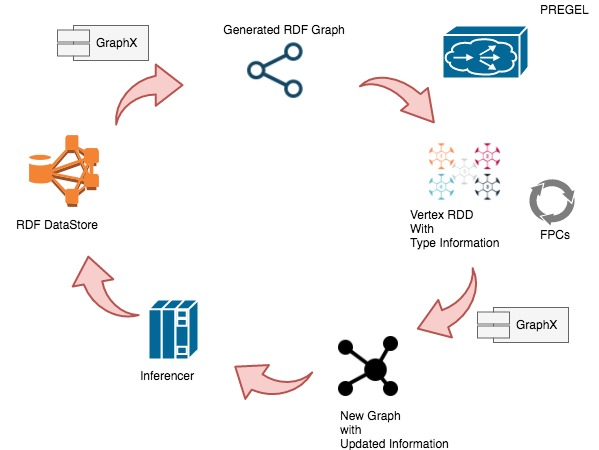
\includegraphics[width=1\textwidth]{RDf2Rule.jpg}
	\caption{The Architecture Overview}
	\label{fig:architecture}
	\end{centering}
\end{figure}

\subsubsection{Pre-processing}
The input to our implementation is an N-triple files containing the triples of RDF data.  We use a small implementation of RDF parser (as per lab exercises) and use it to create a GraphX graph which is used as input for all the subsequent stages.

\subsubsection{Finding Frequent Predicate Cycles (FPCs)}

\paragraph{Original Algorithm}
The original algorithm  finding FPC is to find frequent 1-predicate path, and then repeatedly  find frequent k-predicate paths from the frequent k-1 predicate paths. Algorithm starts a loop that discovers frequent k-predicate paths by extending k-1 predicate paths repeatedly in parallel. For each path  we create an instance of a k-1 predicate path and then on the last element of the path we “smartly” add the new nodes to the path. (Shown in figure). The newly generated set of paths are checked for frequency threshold and in the process of extending predicate paths, the set of last entities in the instance paths are always kept, which facilitates adding new predicates and counting the support of predicate paths.

\paragraph{Implementation}
This approach \cite{tut} was implemented with two different variations using Pregel \cite{nous} (integrated in GraphX) which is a programming model specifically targeted to handle large scale graph problems. The reason behind using Pregel is its ease of programming as  it makes vertices and edges first-class citizens and encourages programmers to think in those terms, rather than in terms of dataflows and transformation operators on parts of the graph. Moreover, the framework is designed to support iterative computations more efficiently than MapReduce, because it keeps the dataset in memory rather than writing it to disk after every iteration. This is useful since many graph algorithms are iterative. It also handles the fact that graph algorithms generally have poor memory access locality, by locating different vertices on different machines and passing messages between machines as necessary.

\begin{itemize}
\item \textbf{Finding FPCs (traditional way)} : The first implementation is theoretically similar to the  original algorithm where we take all possible pairs of nodes in the KB and find all possible paths between them using Pregel. Even though the usage of Pregel makes the path finding faster but taking all possible combination of path makes the algorithm relatively slower. Once all the possible paths are made available they are filtered based on existence of cycles and frequency count of edges occurrence.
\item \textbf{Finding PCs (in one Traversal of Pregel):} The second implementation of the algorithm takes one pass of pregel and is able to locate find all paths for each of the node and create a new VertexRDD which can be replaced in the original graph. We particularly believe that this approach is highly scalable and would result in an enriched knowledge graph in which the type information and path/cycles associated with a resource stored within the vertex and then used easily for frequency count.  However we were unable to count frequency of edge types in the same traversal by pregel as well as facing bugs in mapping the source and destination in the paths.

\end{itemize}

The major challenge and learning from the project is to transform GraphX graph abstraction into a “Vertex like” communication for faster traversal of large scale graph. The pregel follows the following constructor

\begin{lstlisting}
def pregel[A]
      (initialMsg: A,
       maxIter: Int = Int.MaxValue,
       activeDir: EdgeDirection = EdgeDirection.Out)
      (vprog: (VertexId, VD, A) => VD,
       sendMsg: EdgeTriplet[VD, ED] => Iterator[(VertexId, A)],
       mergeMsg: (A, A) => A)
    : Graph[VD, ED]
\end{lstlisting}

The first argument list contains configuration parameters:

\textbf{initialMsg} is the user defined message that will be sent to the vertices prior to superstep 0. \textbf{maxIter} is the maximum number of iterations we will perform before it terminates. \textbf{activeDir} is the  edge direction in which to send messages

The second argument list contains the functions that handles the mutation of state and message passing: \textbf{vprog} is the user defined function for receiving messages.  \textbf{sendMsg} is the user defined function to determine the messages to send out for the next iteration and where to send it to.  \textbf{mergeMsg} is the user defined function to merge multiple messages arriving at the same vertex at the start of a superstep before applying the vertex program vprog.

\subsubsection{Adding Type Information to the Entities in FPCs}

The extraction of type information using pregel is trivial and uses one iteration of the graph and returns the most frequent  type information. The algorithm is implemented similar to the pregel approach for finding PCs.
The following code shows  the way the implementation uses the modified KB graph (output of GraphX) and its attributes to pass the message to be communicated between vertices of the KB and added the type results to the original graph.



\begin{lstlisting}[language=Scala]
val pregelGraph = graph.mapVertices((id, label) => (id, label,
List.empty[String]))
    val messages = pregelGraph.pregel[List[String]](initialMsg,
    maxIterations, activeDirection)
    ((vid, oldMessage, newMessage) => (vid, oldMessage._2, newMessage
     ++ oldMessage._3),
      (triplet) => {
        if (triplet.attr.toString().contains("type"))
          Iterator((triplet.srcId, List(triplet.dstAttr._2)))
        else
          Iterator.empty
      },
      (msg1, msg2) => msg1 ++ msg2)

\end{lstlisting}

In conclusion, the final output of the implementation is an enriched graph in  which each vertex (Resource) contains type information. Further, we also have a list of cycles, which are used for counting all possible edge patterns. Thus, we have successfully achieved the goal of the first two algorithms successfully but there is much more room for improvement.


\subsubsection{Evaluation \& Results}
The system was tested over the implementation on 69,284 triples which was a subset of Semantic Web Dog Food Database.  The testing was done based on a 2.9 Ghz i5 Processor with 8 GB 1867 MHz DDR3 memory.

\begin{table}[htp]
	\begin{centering}
		\begin{tabular}{lr}
		\hline
	    Approach            & Evaluation Time \\
		\hline
		Finding FPCs (traditional way)      &  $\approx$ 18 minutes  \\
		 Finding PCs ( one Traversal of Pregel)  &  $\approx$ 3.6 seconds  \\
	      Finding Type Information (Using Pregel)    &  $\approx$ 2.6 seconds  \\
		\hline
		\end{tabular}
		\caption{Approach 1 Results}
		\label{tab:ltbexample}
	\end{centering}
\end{table}

The results of the FPC algorithm for a Resource with vertex ID 687 is shown as follows. The format of the output  $(<Length of path>, <Type of Edge (Inbound or Outbound )> ; <VertexId> ; <Edge label>; VertexId)$.

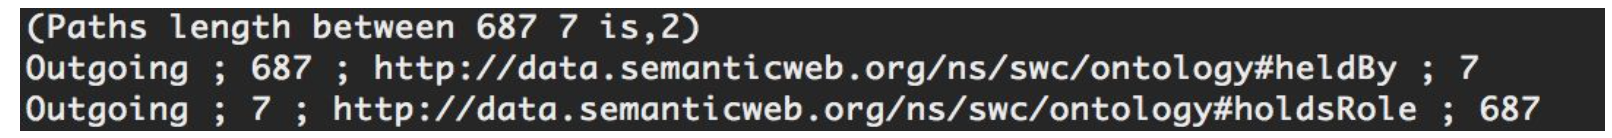
\includegraphics[width=0.9\textwidth]{Fpc.png}

The result of the type Information for a Resource with vertex ID 75 showing the most frequent resource type for this resource.


\includegraphics[width=0.9\textwidth]{typeinfo.png}


\subsection{Approach 2 (GraphX core  Approach)}

\subsubsection{Find Entity Type Information and Update-Graph}
Adding entity type information to rules can produce more accurate rules. For example, without entity type information, we may get rules like $(x1, bornIn, x2) \implies (x1, diedIn, x2)$. Based on this rule, if we already know that someone was born in someplace, then we can predict that this man also died in the same place. However,if the entity instantiating x2 is a small town, the prediction of this rule is prone to be incorrect, because most people would not stay in the same town in their whole lives. If the entity instantiating x2 becomes a country, the prediction will have a higher probability to be correct. Based on this observation, the following rule is more preferable.
Example , $(x1, bornIn, x2) \land (x1, typeOf, People)$ \\
$(x2, typeOf,Country) \implies (x1, die-In, x2)$

\subsubsection{How to Implement it using Spark in Steps: }
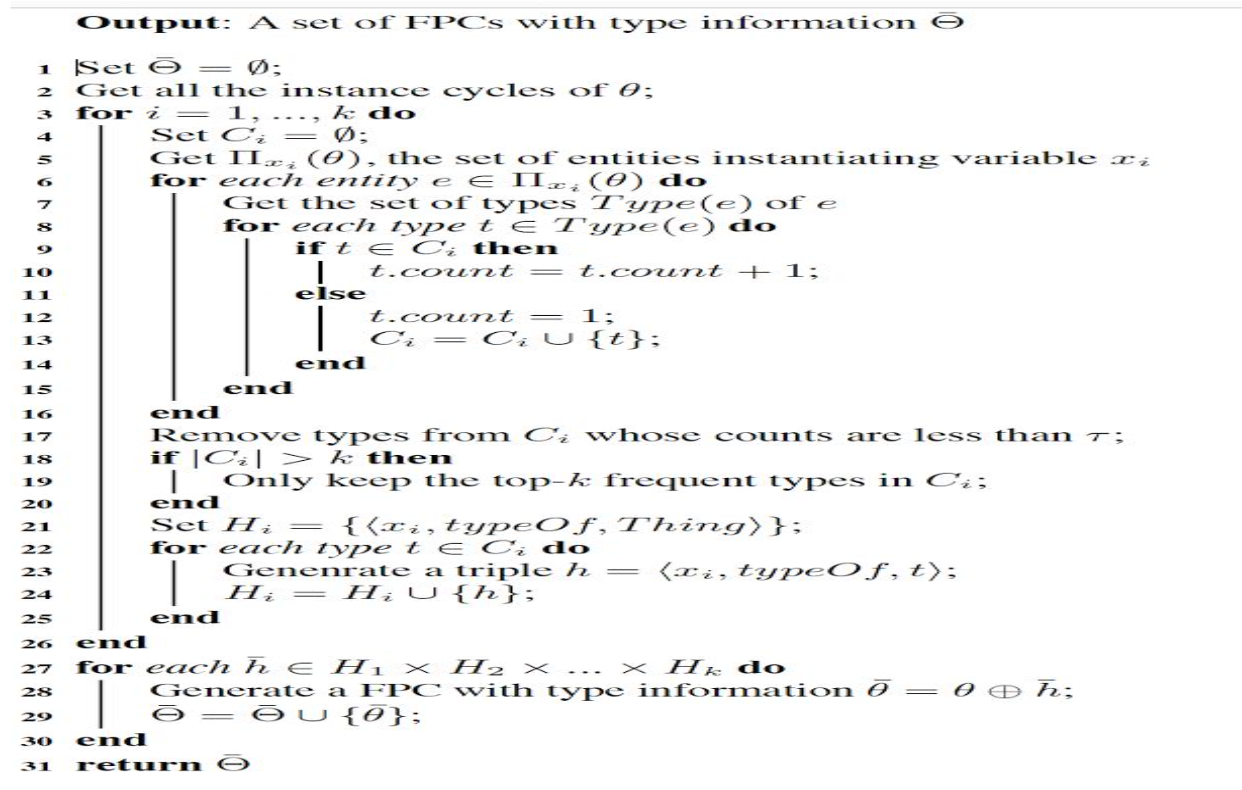
\includegraphics[width=0.9\textwidth]{akhilesh_algo.png}
\begin{enumerate}
\item Line 2: Generate the subgraph  from RDD Graph based on filtering for the given FPCs.
\item Repeat below code for all predicates.
\item Line 5: Get set of entities for given a predicate from FPC
\item Line 6: For loop for each entity can be distributed under graphX RDD .
\item Line 6-16 For a given “Type-of” predicate filter operation we have list of all type list RDD.
\item Line 6-16 Sort All type list RDD according to count to filter for given support count.
\item 17-19 Take only top K frequent predicate .
\item 17-31 Generate edges from  (entity, typeof, frequent-Type) and update graph.

\end{enumerate}

\subsubsection{Advantages(Spark over Algorithm)}
Algorithm works very well on spark distribution wherever you want to do just some transformation and action on the processed graph. (eg. from above para step1, step2-7).

\subsubsection{Disadvantages(Spark over Algorithm)}
Algorithm for updating graph with new edges takes lots of time as it needs to be processed through many iterations. (please find reference in below flow-chart for loop- step 17-31).

\subsubsection{Evaluation}
This algorithm is totally based on frequent type count which is possibly not a better  approach. Eg. (a, type-of, male) and (b, type-of, female ), (male, subclassof, person), (female, subclassof, person). Ideally using frequent type list by this algorithm, you may get possibly a large frequent type for the female candidates. So later while updating graph you need to assign (a, type-of, female) which is already a typeof male . Due to this the rules like $(x1, givesBorn, x2) \land (x1, typeOf, female)\land (x2, typeOf, child) \implies (x1, motherOf, x2)$, will go wrong (depends on frequent support count for person).
\textbf{Solution:} we should consider domain and range of each frequent type before processing it to graph solely based on support count of frequent type.\\

\begin{tabular}{lrrr}
    \hline
     Implementation            & Number of triples & Time   \\
   \hline
    Find Frequent Type (full predicate list )      &  69284 & 1.7 seconds  \\
     Find Frequent Type (full predicate list )      &  1561 & 0.43 seconds  \\
    Updating Graph     &  69284 & 91.7 seconds  \\
    Updating Graph     &  1561 & 4.2 seconds \\

   \hline
  \end{tabular}\\

\emph{Frequent Predicate Type is  not completed due to bad algorithm, taking too much time only for next edge processing. Sublinear time, Brute Force search for next edge. Spark only help while finding frequent type count from database.
}\\

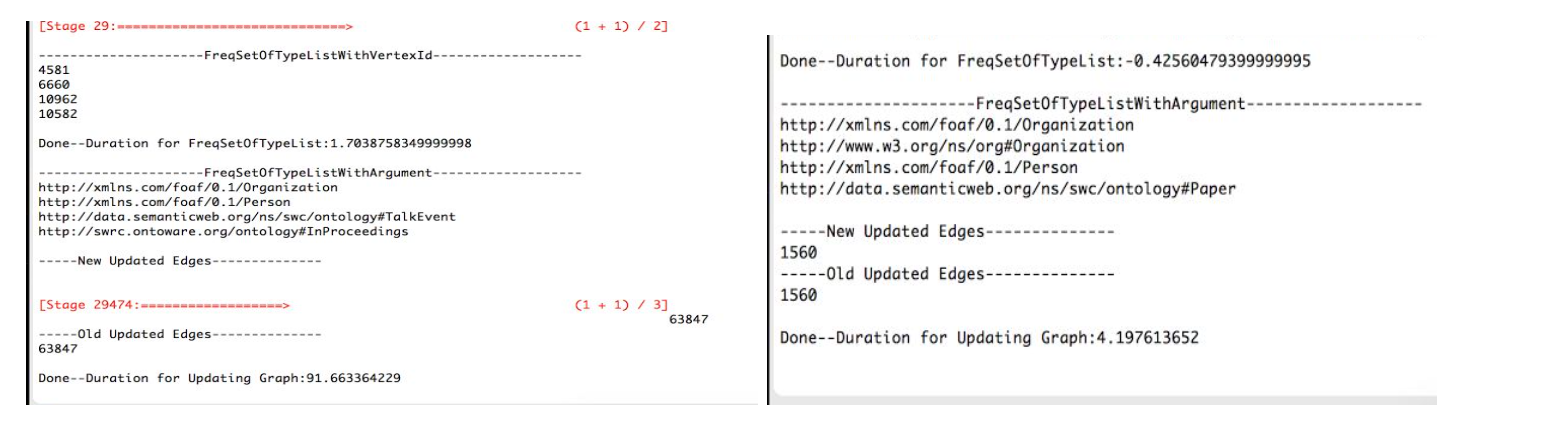
\includegraphics[width=0.9\textwidth]{akhilesh_result.png}
\section{Project Timeline}

\begin{itemize}
    \item \textbf{May 29, 2017 -  June 5, 2017}
    \begin{itemize}
    \item Kunal
    \begin{itemize}
    \item Read the paper.
\item Understood the Algorithm and Divided tasks
 \end{itemize}

 \item Akhilesh
  \begin{itemize}
   \item Read the paper.
\item Understood the Algorithm and Divided tasks
 \end{itemize}

    \end{itemize}

     \item \textbf{June 6, 2017- June 12, 2017}
    \begin{itemize}

    \item Kunal
    \begin{itemize}
    \item Explored all possible features of Spark and GraphX
\item Decided the final technology stack after discussion with mentors
\item Analyzed the portions of algorithm to be improvised / omitted according to the technology stack used.

 \end{itemize}

 \item Akhilesh
  \begin{itemize}
   \item Study of scala-spark language
   \item Understanding of Algorithm in the context of Spark


 \end{itemize}

    \end{itemize}

     \item \textbf{June 13, 2017- June 20, 2017}
    \begin{itemize}

    \item Kunal
    \begin{itemize}
    \item Learned the usage of required API.
\item Implemented Shortest path algorithm using Pregel.
\item Started working on the FPCs.
\item Figured out the type Information can be done using Pregel itself.
\item Prepared the presentation for mid evaluation.
\item Explored improvements in the algorithm for distributed data processing.

 \end{itemize}

 \item Akhilesh
  \begin{itemize}
   \item Learned core graphx API and mapReduce functionality.
\item Implemented entity-Type-Info using graphX APIs
\item Implemented unit test code for entityType Information

 \end{itemize}

    \end{itemize}

     \item \textbf{June 21, 2017- July 17, 2017}
    \begin{itemize}

    \item Kunal
    \begin{itemize}
    \item Finished First Implementation of FPC
\item Evaluated the Implementation
\item Redesigned the algorithm
\item Implemented second implementation of PC.
\item Fixed Bugs in type Information
\item Worked on the  Report (drew the figures for architecture and explained the Pregel methodologies).
\item Discussed the ideas to incorporate frequency count.
\item Studied GraphFrames.

 \end{itemize}

 \item Akhilesh
  \begin{itemize}
   \item Added Type Information to Original Graph Using Graphx.
\item Worked on FPC - frequent subgraph algorithms using core GraphX API  (Not Completed due to its sublinear time or brute force search)
\item Evaluated entity type-Information algorithm advantages and disadvantages with respect to spark.

 \end{itemize}

    \end{itemize}
   \item \textbf{July 18, 2017 – July 25, 2017}
    \begin{itemize}
    \item Kunal
    \begin{itemize}
    \item Prepared the Presentation
\item  Made Final improvements on the report
\item  Wrote the final report in latex.
\item  Had small meetings with various people in trying to look for a solution for the algorithm implementation.

 \end{itemize}
 \item Akhilesh
  \begin{itemize}
   \item Added implementation content to the doc report.
 \end{itemize}
     \end{itemize}
\end{itemize}


%------------------------------------------------------------------------------
\section{Future Work And Improvements}
There are multiple improvisation and extension of the project which we are curious to explore and incorporate into the project. These  are listed as follows:

\begin{enumerate}
\item The FPC generation can be implemented using the Rocha–Thatte Algorithm which is a faster implementation of distributed graph traversal algorithm and much less computational overhead.
\item The type information and the FPC generation (second implementation with correct mapping) can be integrated into one traversal of Graph via Pregel which would result in approximately 2 times the current traversal speeds.
\item Integrate the output into an Inferencing engine.
\item Comparison between the algorithms proposed in 1 and 2 points would also be an interesting insight.
\item Based on the results, in future, the project can be easily exported to work with Data-Frames instead of RDDs and GraphX can be replaced with GraphFrames\cite{graphframes}.

\end{enumerate}


%------------------------------------------------------------------------------

% Refs:
%
\label{sect:bib}
\bibliographystyle{plain}
%\bibliographystyle{alpha}
%\bibliographystyle{unsrt}
%\bibliographystyle{abbrv}
\bibliography{easychair}

\begin{appendices}
\includegraphics[width=0.9\textwidth]{akhilesh_codeflow.jpg}

\end{appendices}
%------------------------------------------------------------------------------
% Index
%\printindex

%------------------------------------------------------------------------------
\end{document}

% EOF
